% Created 2024-07-22 Mon 09:55
% Intended LaTeX compiler: pdflatex
\documentclass[letterpaper, 12pt]{article}
\usepackage[utf8]{inputenc}
\usepackage[T1]{fontenc}
\usepackage{graphicx}
\usepackage{longtable}
\usepackage{wrapfig}
\usepackage{rotating}
\usepackage[normalem]{ulem}
\usepackage{amsmath}
\usepackage{amssymb}
\usepackage{capt-of}
\usepackage{hyperref}
\usepackage{minted}
\usepackage{xcolor}
\usepackage{hyperref}
\usepackage{tocloft}
\usepackage{minted}
\usemintedstyle{manni}
\usepackage{pdfpages}
\usepackage{fancyhdr}
\usepackage{graphicx}
\usepackage[top=1.4in, left=0.5in, right=0.5in, bottom=0.8in]{geometry}
\usepackage[T1]{fontenc}
\usepackage{helvet}
\pagestyle{fancy}
\renewcommand{\headrulewidth}{0pt}
\renewcommand{\footrulewidth}{0pt}
\setlength{\parindent}{0em}
\setlength{\parskip}{1em}
\usepackage{hyperref}
\usepackage {color}
\usepackage {tabularray}
\usepackage{xcolor}
\hypersetup{
colorlinks=true,
linkcolor=blue,
filecolor=magenta,
urlcolor=cyan,
citecolor=green,
pdfborder={0 0 0}
}
\usepackage[most]{tcolorbox}
\author{Hilduara Abreu}
\date{\today}
\title{Parent Notification Letter for Schools Designated for LSI\\\medskip
\large school leters to parents}
\hypersetup{
 pdfauthor={Hilduara Abreu},
 pdftitle={Parent Notification Letter for Schools Designated for LSI},
 pdfkeywords={},
 pdfsubject={},
 pdfcreator={Emacs 29.3 (Org mode 9.8)}, 
 pdflang={English}}
\begin{document}

\fancyfoot[C]{\setlength{\unitlength}{1in}\begin{picture}(5,0)\put(-1.8,-0.5){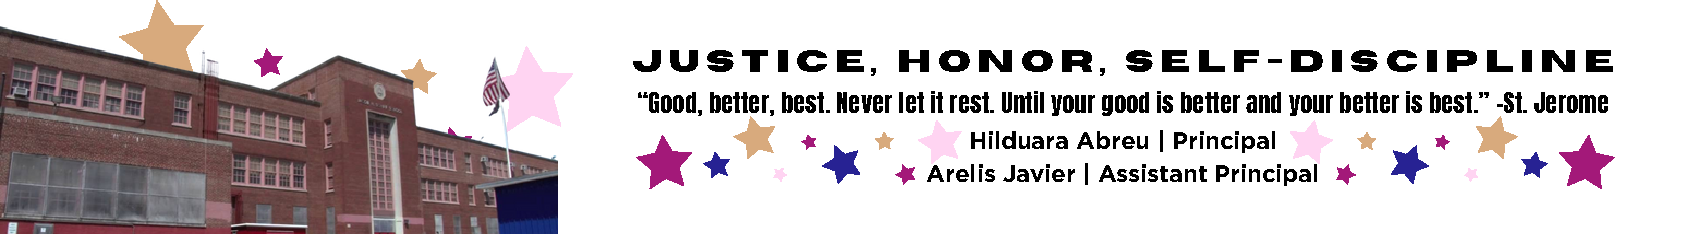
\includegraphics[width=8.8in,height=1.3in]{logo-1}}\end{picture}}
\fancyhead[C]{\setlength{\unitlength}{1in}\begin{picture}(5,0)\put(-1.9,-0.5){
\includegraphics[width=8.9in,height=1.3in]{logo-2}}\end{picture}}
\fancyhead[R]{\thepage}
\pagenumbering{gobble}

\begin{document}
\vspace*{0.1in}
Date: \href{https://www.ps192.org/apps/bbmessages/show_bbm.jsp?REC_ID=139439}{February 16, 2024}

Subject: \textbf{Parent Notification Letter For schools Designated For LSI}

Dear Parent or Guardian,

This letter is to notify you that, our school,Jacob H. Schiff | PS 192, has been
designated for Local Support and Improvement (LSI) by the New York State
Education Department (NYSED) for the 2023-24 school year based on the performance of our students on New York State assessments in school year 2022-23. The
designation “Local Support and Improvement (LSI),” recognizes that all schools,
even higher performing schools like ours, are in a continuous improvement mode
and can benefit from local support from their districts to meet students’ differentiated needs. LSI or “Good Standing” is the best accountability status
currently available. The school’s designation is part of the state’s
accountability system consistent with federal Elementary and Secondary Education Act (ESEA) requirements.

I’m confident that the programs and interventions that are being implemented
citywide and at our school will continue to make the 2023-24 school year a high-quality educational experience for your child.

Thank you for your ongoing partnership and support. Our entire school staff is
committed to ensuring a successful year for our students and school community.
If you have any questions or concerns, please feel free to contact me at 212-775-9560.

Sincerely,


\includegraphics[width=100px,height=50px]{hil_signature.png}

\textbf{Hilduara Abreu}

\textbf{Principal}

\textit{The School of Joyful Learning!}

\href{https://www.ps192.org}{www.ps192.org}

\tcbuselibrary{}
\newtcolorbox{bluebox}[1][]{
  colback=blue!5!white,
  colframe=blue!75!black,
  fonttitle=\bfseries,
  coltitle=black,
  enhanced,
  attach boxed title to top center={yshift=-2mm},
  title=#1,
  boxed title style={colback=blue!50!white}
}
\newtcolorbox{greenbox}[1][]{
  colback=green!5!white,
  colframe=green!75!black,
  fonttitle=\bfseries,
  coltitle=black,
  enhanced,
  attach boxed title to top center={yshift=-2mm},
  title=#1,
  boxed title style={colback=green!50!white}
}
\newtcolorbox{redbox}[1][]{
  colback=red!5!white,
  colframe=red!75!black,
  fonttitle=\bfseries,
  coltitle=black,
  enhanced,
  attach boxed title to top center={yshift=-2mm},
  title=#1,
  boxed title style={colback=red!50!white}
}
\end{document}
